%----------------------------------------------------------------------------
\chapter{Programok, technológiák bemutatása} \label{fejezet2}
%----------------------------------------------------------------------------

\section {Az alkalmazás felépítése}

\subsection{Frontend}

A frontend fejlesztéséhez HTML-t, CSS-t és JavaScriptet használtam, amelyek lehetővé teszik az interaktív felhasználói felület létrehozását és a dinamikus funkcionalitás implementálását. Ezek a technológiák biztosítják a felhasználók számára az intuitív böngészési élményt és a kriptográfiai rendszerek kipróbálását.
Valamint a Jinja2 sablonmotort használtam, hogy segítsen a dinamikus tartalmú weboldalak generálásával, amelynek használatát egy külön szekcióba fejtem ki. (\ref{sec:jinja2})

\textbf{HTML:}
Egy szabványosított jelölőnyelv, amelyet a weboldal strukturálására és tartalma megjelenítésére használtam. Segítségével definiáltam az elemeket, például címeket, szövegeket, képeket, hivatkozásokat stb.

\textbf{CSS:}
Egy stílusleíró nyelv, amelyet a weboldal megjelenítési formázására használtam. Azáltal, hogy különböző stílusokat és tulajdonságokat adtam meg az elemeknek, mint például a szín, a betűtípus, a méret, a margók, a pozíció stb., a CSS lehetővé tette a weboldal testreszabását és a vizuális vonzereje növelését.

\textbf{JavaScript:}
Egy programozási nyelv, amelyet az alkalmazás interaktív funkcióinak megvalósítására használtam. A JavaScript lehetővé teszi a weboldalam dinamikus működését, a felhasználói interakciókat, az adatok feldolgozását és a weboldalhoz kapcsolódó események kezelését.

\begin{figure}[!h]
	\centering
	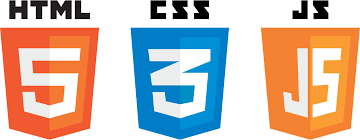
\includegraphics[scale=0.3]{images/logoHtmlCssJs}
	\caption{HTML - CSS - JS logók}
\end{figure}


\newpage
\subsection{Backend}

Backend oldalon a szerveroldali programozáshoz a Python programozási nyelvet választottam, amely nagy népszerűségnek örvend Flask keretrendszerrel kombinálva. A Python és a Flask együtt lehetővé teszik a hatékony és gyors fejlesztést, valamint az API-k létrehozását és a kérések kezelését.

Az adatbázis kezeléséhez az SQLAlchemy nevű Python könyvtárat használtam, melynek segítségével könnyedén lehet adatmodelleket definiálni és adatbázisműveleteket végezni. Ezáltal hatékony és strukturált adatkezelést biztosít az alkalmazásban.

Ezen technológiák kombinációja lehetővé teszi az alkalmazás teljeskörű működését, az interaktív felhasználói felülettől kezdve az adatok kezeléséig és tárolásáig. Az alkalmazás fejlesztése során a modern frontend és backend technológiák összekapcsolása révén egy hatékony és felhasználóbarát környezetet hoztam létre a kriptográfiai rendszerek kipróbálásához és tanulásához.

\vspace{10pt}
\textbf {Python:}
A Python egy magas szintű programozási nyelv, amelyet egyszerű és olvasható szintaxisa jellemez. A Python nagyon rugalmas és sokoldalú, és széles körben használják a webfejlesztés, adatelemzés, mesterséges intelligencia, gépi tanulás és sok más területen. A Pythonban kifejezőerő és kényelem találkozik, ami lehetővé teszi a gyors és hatékony fejlesztést. Emellett a Python gazdag könyvtárökoszisztémával rendelkezik, amely számos előre elkészített funkcióval és modullal bővíti a fejlesztési lehetőségeket.

\vspace{10pt}
\textbf {Flask:}
A Flask egy könnyűsúlyú és rugalmas webes keretrendszer Pythonban. A Flask lehetővé teszi a webalkalmazások gyors és hatékony fejlesztését, minimális konfigurációval és egyszerű szintaxisával. A Flask kiváló választás olyan projektekhez, amelyek kisebb méretűek vagy kevesebb komplexitást igényelnek, ugyanakkor rugalmasságot és skálázhatóságot biztosítanak. A Flask lehetőséget nyújt a beépített funkciók, mint például útvonalak, nézetek, sablonok és adatbázis kezelése egyszerű implementálására.

\vspace{10pt}
\textbf {SQLAlchemy:}
Az SQLAlchemy egy Python alapú ORM (Object-Relational Mapping) keretrendszer, amely lehetővé teszi az adatbázisokhoz való könnyű és hatékony hozzáférést. Az ORM segítségével a fejlesztők Python objektumokat tudnak kezelni és manipulálni, miközben azokat az adatbázisban tárolják. Ezáltal az SQLAlchemy elrejti az adatbázis-specifikus részleteket és absztrakciós réteget biztosít a programozó számára.

\pagebreak
\begin{figure}[!h]
	\centering
	
\includegraphics[scale=0.15]{images/logoPythonFlaskSqlalchemy}
	\caption{Python - Flask - SQLAlchemy logók}
\end{figure}


\section {Hasonló platformok, szoftverek összehasonlítása}

\textbf{Cryptii \cite{Cryi}:} A Cryptii egy online titkosítási és dekódolási weboldal, amely algoritmusok széles skáláját támogatja. Különböző szimmetrikus és aszimmetrikus titkosítási algoritmusok közül választhat. A weboldal emellett lehetőséget biztosít a kódolásra, a hashelésre és a tömörítésre is. A bevitel és kimenet között lehetőség van különböző rétegeket beiktatni, így a két végpont között több algoritmus is alkalmazható.

\textbf{Encode-Decode \cite{EnDe}:} Az Encode-Decode egy olyan weboldal, amely különböző algoritmusokhoz kínál titkosítási és dekódolási szolgáltatásokat. A weboldal egy egyszerű felületet biztosít, ahol beírhatja a szöveget, és kiválaszthatja a kívánt titkosítási vagy visszafejtési módszert.

A Cryptii és Encode-Decode platform sem ad leírást a használt algoritmusokról, így ezeket csak úgy lehet hatékonyan használni amennyiben ismerjük azokat, vagy más forrásokból tájékozódunk róluk.

\vspace{10pt}
\textbf{CyberChef \cite{CyCh}:} A CyberChef egy hatékony online eszköz az adatmanipulációhoz és a titkosításhoz/dekódoláshoz. A műveletek széles skáláját kínálja, beleértve az olyan titkosítási algoritmusokat, mint az AES, RSA, XOR és még sok más. Támogatja továbbá a kódolást, a hashelést, a tömörítést és más adattranszformációkat.

\textbf{Rumkin \cite{Rum}:} A Rumkin egy olyan weboldal, amely kriptográfiai eszközök széles gyűjteményét kínálja. Különböző algoritmusokhoz kínál lehetőségeket, mint például a Caesar rejtjelezés, a Rail Fence rejtjelezés, a Playfair rejtjelezés és még sok más. Emellett kódolásra, hashelésre és steganográfiára szolgáló eszközöket is tartalmaz.

\textbf{dCode \cite{dCo}:} A dCode egy olyan online platform, amely titkosítási és dekódolási eszközök hatalmas gyűjteményét kínálja. Algoritmusok, titkosítások és kódolások széles skáláját fedi le, beleértve a klasszikus titkosításokat, modern titkosítási módszereket és speciális kódolásokat. Emellett kriptoanalízishez is kínál eszközöket.

Az utolsó három alkalmazás esetében már több, részletesebb leírást lehet kapni az algoritmusokról, bár már kevésbé felhasználóbarátok, mint az első két platform.


